\chapter{الفلزات: تفاعلاتها مع الأحماض وتآكلها}\label{ch:g9:metals-acids-corrosion}

في الميناء، يتخطط الهيكل الفولاذي لقارب صيد قديم \omterm{def:g9:metals-acids-corrosion:corrosion}{بصدأ} برتقالي. وعلى الرصيف
بوابة مكسوة بالزنك وقفت تحت المطر ثلاثين سنة ولا تزال تلمع لمعانًا رماديًا
باهتًا. وفي المتحف خاتم من الذهب دُفن ثلاثة آلاف سنة يبرق كيوم صُنع. فالفلزات
لا تواجه العالم كلها بالطريقة نفسها: بعضها يهاجمه الماء \omterm{def:g4:air-a-mixture-of-gases:air}{والهواء} والأحماض،
وبعضها لا يكاد يتأثر.

\begin{recall}
\omterm{def:g9:ions:ion}{الأيونات} \omterm{def:g7:atoms-and-molecules:atom}{ذرات} مشحونة؛ والفلزات تعطي كاتيونات مثل \ce{Fe^{2+}}
و\ce{Zn^{2+}} و\ce{Al^{3+}}، يُتعرّف عليها باختبارات الترسيب
(\cref{ch:g9:ions}). \omterm{def:g9:acids-bases-ph:acidic}{والمحلول الحمضي} يحوي \omterm{def:g9:ions:ion}{أيونات} \ce{H+(aq)} كثيرة
(\cref{ch:g9:acids-bases-ph}). والهيدروجين يحترق بفرقعة حادة عند فوهة
أنبوب الاختبار (\cref{ch:g7:identifying-substances}).
\end{recall}

\begin{omfigure}
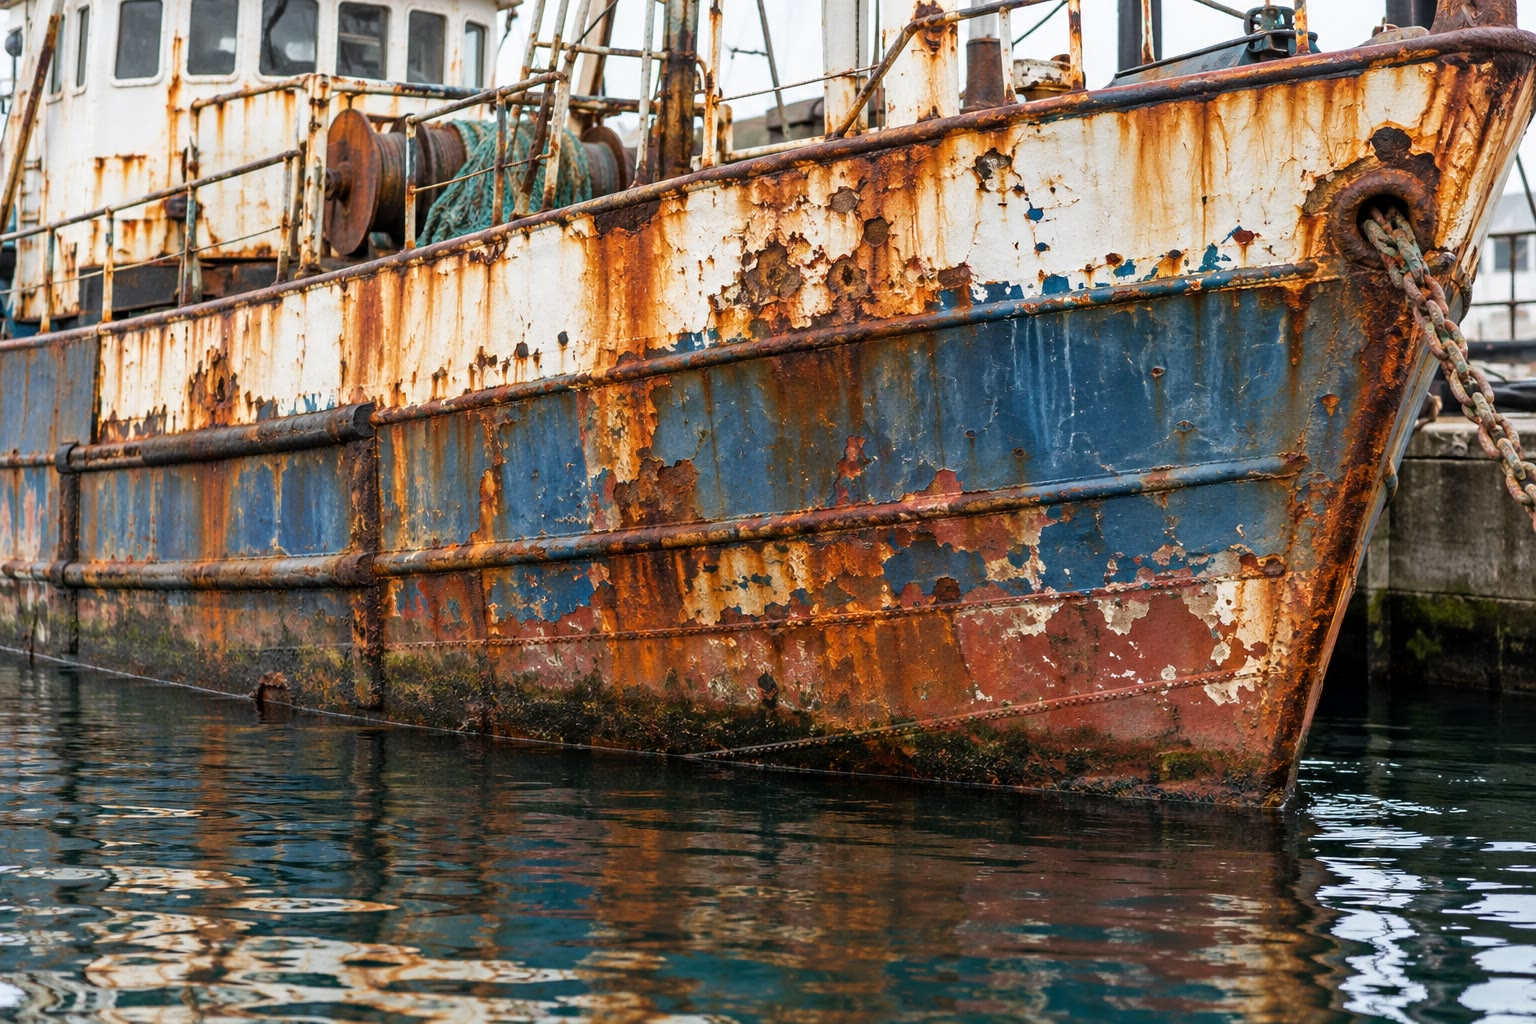
\includegraphics[width=0.55\linewidth]{images/book1/ai/g9-rusty-hull.jpg}

{\small هيكل قارب قديم: الفولاذ يصدأ.}
\end{omfigure}

\section{الفلزات في حمض الهيدروكلوريك}

\begin{inthelab}[ثلاثة فلزات في حمض]
يُسقط المعلم قطعة صغيرة من الحديد، وأخرى من الزنك، وثالثة من النحاس في ثلاثة
أنابيب اختبار فيها حمض الهيدروكلوريك المخفف. فتصعد الفقاعات من الحديد
والزنك، ببطء من الحديد، وبنشاط من الزنك، ويختفي الفلزان شيئًا فشيئًا؛ ولا يحدث
شيء للنحاس. والغاز، إذا جُمع في أنبوب صغير، يُحدث فرقعة حادة: إنه
الهيدروجين. ومع هيدروكسيد الصوديوم يعطي سائل الأنبوب الأول راسبًا أخضر
(\omterm{def:g9:ions:ion}{أيونات} \ce{Fe^{2+}})، وسائل الثاني راسبًا أبيض (\omterm{def:g9:ions:ion}{أيونات} \ce{Zn^{2+}}).
\end{inthelab}

\begin{omfigure}
\begin{tikzpicture}[font=\small, scale=1.2]
  \foreach \k/\m/\c/\bub in {0/{حديد}/black!45/4, 1/{زنك}/black!25/9, 2/{نحاس}/orange!60!brown/0} {
    \pic[transform shape] at (\k*2.4,0) {testtube={0.55}{omWater!70}};
    \fill[\c] (\k*2.4-0.13,0.08) rectangle (\k*2.4+0.13,0.35);
    \ifnum\bub>0
      \foreach \j in {1,...,\bub} {
        \pgfmathsetmacro\yy{0.45+0.12*\j}
        \pgfmathsetmacro\xx{\k*2.4+0.1*sin(97*\j)}
        \draw[black!55] (\xx,\yy) circle (0.035);
      }
    \fi
    \node[anchor=north, align=center] at (\k*2.4,-0.15) {\m};
  }
  \node[anchor=north, align=center, font=\footnotesize] at (0,-0.6) {فقاعات، ببطء};
  \node[anchor=north, align=center, font=\footnotesize] at (2.4,-0.6) {فقاعات، بنشاط};
  \node[anchor=north, align=center, font=\footnotesize] at (4.8,-0.6) {لا تفاعل};
\end{tikzpicture}

{\small الحديد والزنك والنحاس في حمض الهيدروكلوريك المخفف: الحديد والزنك
يطلقان الهيدروجين؛ والنحاس لا يتفاعل.}
\end{omfigure}

\begin{proposition}[فلز مع حمض]\label{prop:g9:metals-acids-corrosion:acid}
كثير من الفلزات --- الحديد، والزنك، والألومنيوم، والمغنيسيوم --- يتفاعل مع
\omterm{def:g9:ions:ion}{أيونات} \ce{H+} في الحمض: فيختفي الفلز على هيئة \omterm{def:g9:ions:ion}{أيونات} فلزية تبقى ذائبة،
وينطلق غاز الهيدروجين. أما النحاس والفضة والذهب فلا تتفاعل مع حمض
الهيدروكلوريك.
\end{proposition}

\section{كتابة المعادلة بالأيونات}

\begin{definition}[الأيون المتفرج]\label{def:g9:metals-acids-corrosion:spectator}
\omterm{def:g9:ions:ion}{الأيون} الموجود في \omterm{def:g2:mixing-and-dissolving:dissolve}{المحلول} في أثناء التفاعل دون أن يشارك فيه، والذي نجده في
النهاية دون تغيير، هو \emph{أيون
متفرج}\index{أيون متفرج}. ولا يُكتب في المعادلة.
\end{definition}

\begin{example}[الحديد والزنك في حمض الهيدروكلوريك]\label{ex:g9:metals-acids-corrosion:iron}
يحوي حمض الهيدروكلوريك \omterm{def:g9:ions:ion}{أيونات} \ce{H+(aq)} و\ce{Cl-(aq)}. ونجد \omterm{def:g9:ions:ion}{أيونات}
الكلوريد في النهاية دون تغيير: فهي \omterm{def:g9:ions:ion}{أيونات} متفرجة. والمعادلتان
هما
\[
  \ce{Fe(s) + 2H+(aq) -> Fe^{2+}(aq) + H2(g)}, \qquad
  \ce{Zn(s) + 2H+(aq) -> Zn^{2+}(aq) + H2(g)}.
\]
وهما موزونتان في \omterm{def:g7:atoms-and-molecules:atom}{الذرات} وفي الشحنات معًا: $+2$ في كل طرف.
\end{example}

\begin{method}[كتابة معادلة تفاعل فلز مع حمض]\label{met:g9:metals-acids-corrosion:write}
\begin{enumerate}
  \item \omterm{def:g7:chemical-reactions:reactant}{المتفاعلات}: الفلز (s) \omterm{def:g9:ions:ion}{وأيونات} \ce{H+(aq)}.
  \item \omterm{def:g7:chemical-reactions:reactant}{النواتج}: \omterm{def:g9:ions:ion}{أيون} الفلز (aq)، بشحنته المعتادة،
        والهيدروجين \ce{H2(g)}.
  \item وازن \omterm{def:g7:atoms-and-molecules:atom}{الذرات}، ثم تحقق من أن الشحنة الكلية واحدة
        في الطرفين.
\end{enumerate}
وللألومنيوم: \ce{2Al(s) + 6H+(aq) -> 2Al^{3+}(aq) + 3H2(g)}؛ والشحنة
$+6$ في كل طرف.
\end{method}

\begin{safety}{\ghs[0.8cm]{GHS02}\ghs[0.8cm]{GHS04}}
% ledger: ghs:H2
الهيدروجين المنطلق شديد القابلية للاشتعال. ويُجري المعلم التفاعل في أنابيب
اختبار صغيرة، بعيدًا عن أي لهب ما عدا اللهب المستعمل في اختبار
الفرقعة.
\end{safety}

\section{التآكل}

\begin{definition}[التآكل والصدأ]\label{def:g9:metals-acids-corrosion:corrosion}
\emph{التآكل}\index{تآكل} هجوم بطيء على فلز من المواد المحيطة به ---
الأكسجين، والماء، والأحماض، والأملاح --- يحوّل الفلز إلى \omterm{def:g9:ions:ion}{أيونات} أو إلى مركبات
مثل الأكاسيد. وتآكل الحديد والفولاذ يُنتج \emph{الصدأ}\index{صدأ}، وهو أكسيد
حديد مميّه بني هشّ، يتقشر فيسمح للهجوم بأن يمضي إلى
الأعمق.
\end{definition}

\begin{proposition}[ما يحتاجه الحديد ليصدأ]\label{prop:g9:metals-acids-corrosion:needs}
لا يصدأ الحديد إلا إذا وصل إليه الأكسجين والماء معًا. والملح الذائب في
الماء، كما على الطرق المملّحة في الشتاء أو عند البحر، يسرّع
\omterm{def:g9:metals-acids-corrosion:corrosion}{الصدأ}.
\end{proposition}

\begin{inthelab}[ثلاثة مسامير، أسبوع واحد]
توضع ثلاثة مسامير حديد نظيفة في ثلاثة أنابيب اختبار: الأول مع \omterm{def:g4:air-a-mixture-of-gases:air}{هواء} جاف ومادة
مجففة تزيل بخار الماء؛ والثاني في ماء مغلي لإزالة \omterm{def:g4:air-a-mixture-of-gases:air}{الهواء} الذائب فيه، تغطيه
طبقة من الزيت؛ والثالث نصفه في ماء الصنبور ونصفه في \omterm{def:g4:air-a-mixture-of-gases:air}{الهواء}. وبعد أسبوع
لا يكون صدئًا إلا المسمار الثالث.
\end{inthelab}

\begin{omfigure}
\begin{tikzpicture}[font=\small, scale=1.2]
  % tube 1: dry air, drying agent
  \pic[transform shape] at (0,0) {testtube={0.18}{white!80!black}};
  \foreach \x/\y in {-0.12/0.15,0.08/0.12,-0.02/0.3,0.12/0.32,-0.14/0.42,0.03/0.48}
    \fill[black!35] (\x,\y) circle (0.05);
  \fill[black!45] (-0.03,1.0) rectangle (0.03,2.4);
  \fill[black!45] (-0.09,2.4) rectangle (0.09,2.48);
  \fill[black!60] (-0.3,2.8) rectangle (0.3,3.1);
  \node[anchor=north, align=center] at (0,-0.15) {هواء جاف:\\ لا صدأ};
  % tube 2: boiled water under oil
  \pic[transform shape] at (2.6,0) {testtube={0.7}{omWater!80}};
  \fill[yellow!55!orange!60] (2.36,1.85) rectangle (2.84,2.1);
  \fill[black!45] (2.57,0.3) rectangle (2.63,1.7);
  \fill[black!45] (2.51,1.7) rectangle (2.69,1.78);
  \fill[black!60] (2.3,2.8) rectangle (2.9,3.1);
  \node[anchor=north, align=center] at (2.6,-0.15) {ماء بلا هواء:\\ لا صدأ};
  % tube 3: water and air
  \pic[transform shape] at (5.2,0) {testtube={0.4}{omWater!80}};
  \fill[black!45] (5.17,0.3) rectangle (5.23,2.2);
  \fill[black!45] (5.11,2.2) rectangle (5.29,2.28);
  \fill[orange!60!brown] (5.15,0.9) rectangle (5.25,1.5);
  \node[anchor=north, align=center] at (5.2,-0.15) {ماء وهواء:\\ صدأ};
  \draw[<-, omProp, thick] (-0.15,0.3) -- (-0.9,0.7) node[left, text=black, font=\footnotesize] {مادة مجففة};
  \draw[<-, omProp, thick] (2.85,1.98) -- (3.6,2.4) node[right, text=black, font=\footnotesize] {زيت};
\end{tikzpicture}

{\small تجربة المسامير الثلاثة: لا يصدأ الحديد إلا حيث يصل إليه الماء
والأكسجين معًا، وهنا عند سطح الماء.}
\end{omfigure}

\begin{example}[الألومنيوم والنحاس يحميان نفسيهما]\label{ex:g9:metals-acids-corrosion:protect}
يهاجم أكسجين \omterm{def:g4:air-a-mixture-of-gases:air}{الهواء} الألومنيوم في الحال، لكن طبقة الأكسيد الرقيقة المتكوّنة
تلتصق بالفلز وتعزله عن \omterm{def:g4:air-a-mixture-of-gases:air}{الهواء}: فأطر النوافذ الألومنيوم تدوم عقودًا. والنحاس،
الذي يهاجمه \omterm{def:g4:air-a-mixture-of-gases:air}{الهواء} والماء وثنائي أكسيد الكربون ببطء، يتغطى بقشرة خضراء، هي
الزنجار، تلتصق هي أيضًا وتحمي الفلز تحتها. أما \omterm{def:g9:metals-acids-corrosion:corrosion}{الصدأ} فيتقشر على
العكس.
\end{example}

\begin{omfigure}
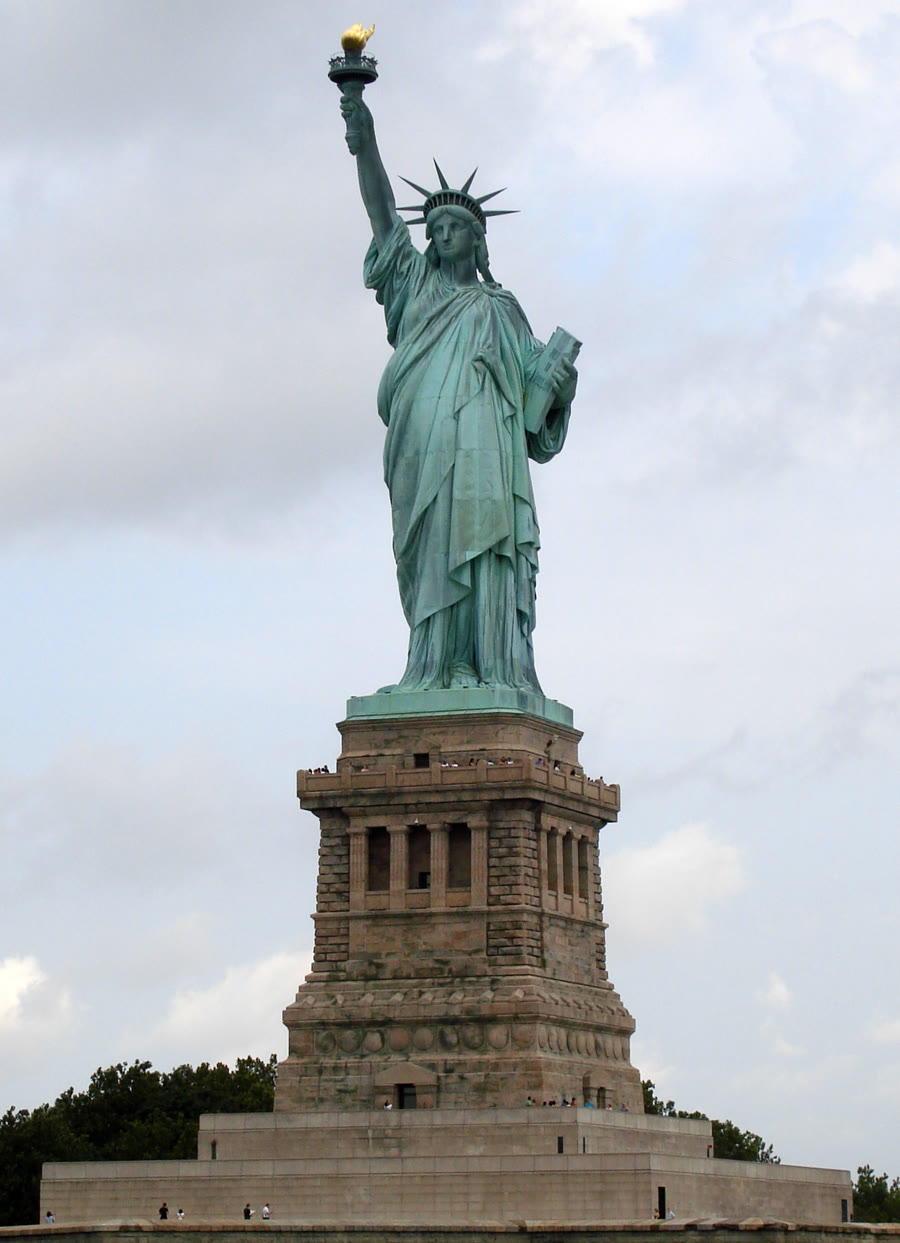
\includegraphics[height=6cm]{images/book1/statue-patina.jpg}

{\small تمثال الحرية: جلده النحاسي مغطى بزنجار أخضر. تصوير: Elcobbola،
ملك عام.}
\end{omfigure}

\section{حماية الفلزات}

\begin{definition}[الغلفنة]\label{def:g9:metals-acids-corrosion:galvanising}
\emph{الغلفنة}\index{غلفنة} كسو الفولاذ بطبقة من الزنك، بغمسه في الزنك
المنصهر. \omterm{def:g4:air-a-mixture-of-gases:air}{فالهواء} والماء يهاجمان الزنك بدلًا من الفولاذ الذي تحته: وحتى حيث
يُخدش الغلاف يتآكل الزنك المجاور أولًا ويسلم الفولاذ.
\end{definition}

\begin{proposition}[طرائق حماية الحديد والفولاذ]\label{prop:g9:metals-acids-corrosion:ways}
\begin{itemize}
  \item إبعاد الماء \omterm{def:g4:air-a-mixture-of-gases:air}{والهواء}: الطلاء، والزيت، والشحم، والغلاف البلاستيكي؛
  \item \omterm{def:g9:metals-acids-corrosion:galvanising}{الغلفنة}: طبقة من الزنك تتآكل بدلًا من الفولاذ؛
  \item استعمال الفولاذ المقاوم \omterm{def:g9:metals-acids-corrosion:corrosion}{للصدأ}، وهو سبيكة من الحديد والكروم تحمي
        نفسها بطبقة أكسيد رقيقة عازلة؛
  \item تثبيت كتل من الزنك على هياكل السفن: فيتآكل الزنك ببطء بدلًا من
        الفولاذ، ويُستبدل من حين إلى آخر (ويُشرح كيف يحدث ذلك في أحد
        كتب المرحلة الجامعية).
\end{itemize}
\end{proposition}

\begin{omfigure}
\begin{minipage}[b]{0.52\linewidth}\centering
\begin{tikzpicture}[font=\small]
  \fill[black!35] (0,0) rectangle (5,0.8);
  \fill[black!15] (0,0.8) rectangle (2.2,1.1);
  \fill[black!15] (2.8,0.8) rectangle (5,1.1);
  \fill[omWater!80] (1.6,1.1) rectangle (3.4,1.35);
  \fill[omWater!80] (2.2,0.8) rectangle (2.8,1.1);
  \draw[black!60] (0,0) rectangle (5,0.8);
  \foreach \x in {1.95,2.1} \draw[->, omProp, thick] (\x,1.25) -- (\x+0.05,1.7);
  \node[anchor=west, font=\footnotesize] at (5.1,0.4) {فولاذ};
  \node[anchor=west, font=\footnotesize] at (5.1,0.95) {طبقة زنك};
  \node[anchor=south, font=\footnotesize, align=center] at (2.0,1.75) {أيونات الزنك\\ تذهب إلى الماء};
  \node[anchor=north, font=\footnotesize, align=center] at (2.5,-0.05) {خدش: ينكشف الفولاذ،\\ لكن الزنك المحيط به\\ يتآكل أولًا};
\end{tikzpicture}

{\small صفيحة مغلفنة مخدوشة.}
\end{minipage}\hfill
\begin{minipage}[b]{0.44\linewidth}\centering
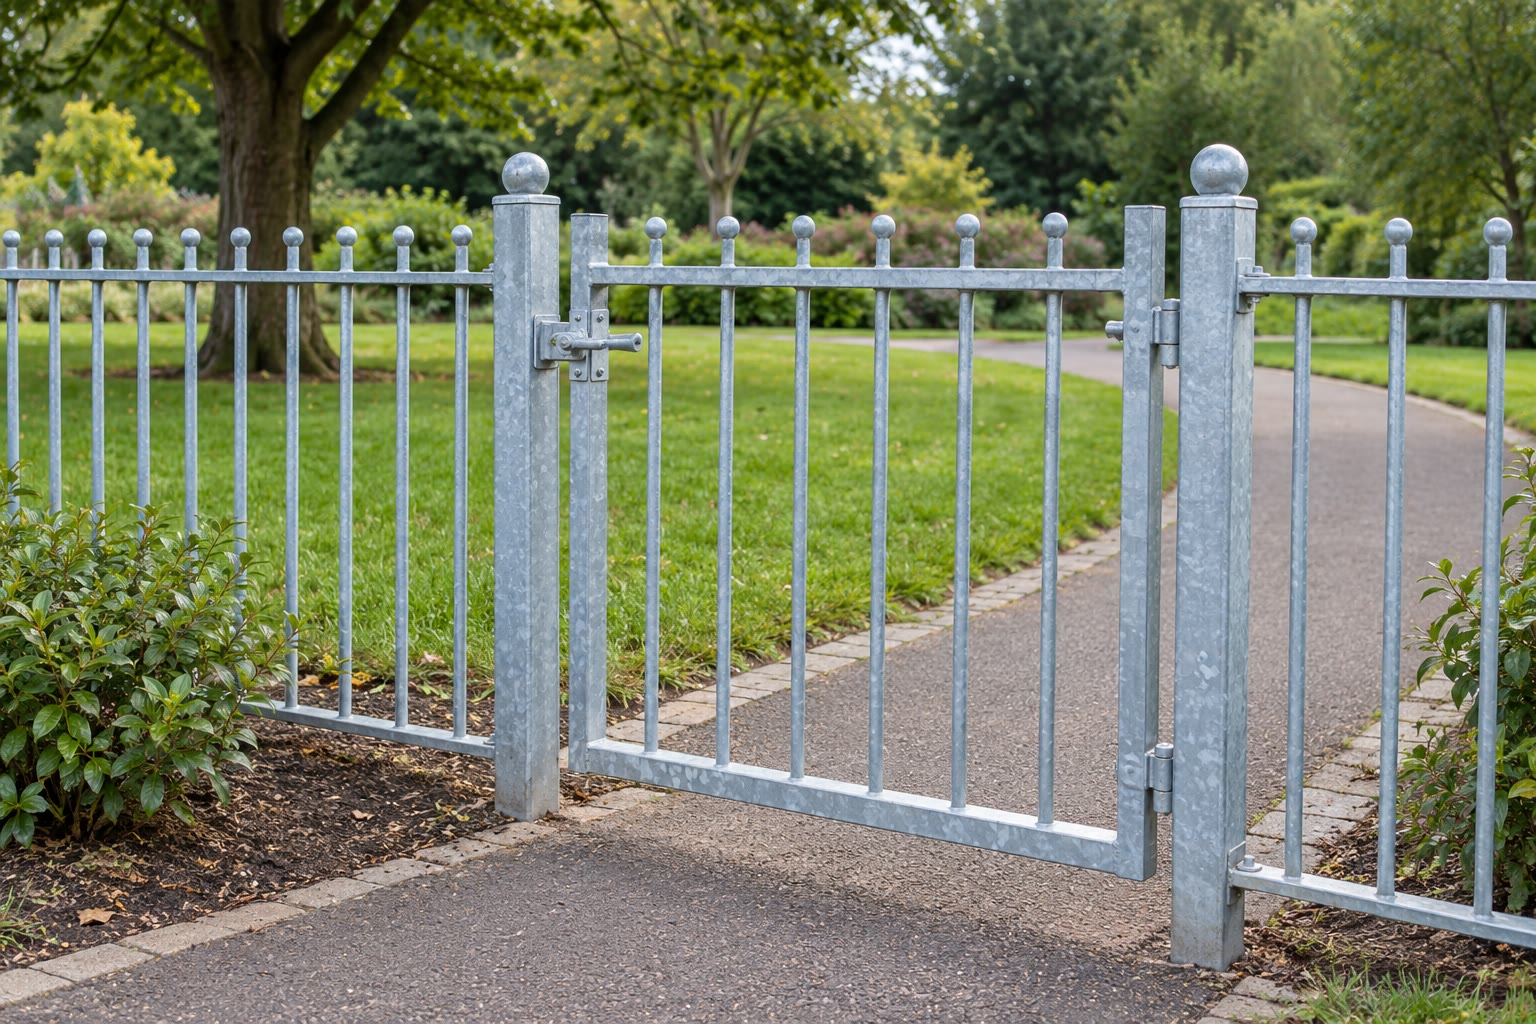
\includegraphics[width=\linewidth,height=4.4cm,keepaspectratio]{images/book1/ai/g9-galvanised-railings.jpg}

{\small درابزين من الفولاذ المغلفن.}
\end{minipage}
\end{omfigure}

\section{تمارين}

\begin{exercise}[$\star$]\label{exo:g9:metals-acids-corrosion:1}
أي غاز ينطلق حين يتفاعل الزنك مع حمض الهيدروكلوريك؟ وكيف يُتعرّف
عليه؟
\end{exercise}

\begin{exercise}[$\star$]\label{exo:g9:metals-acids-corrosion:2}
أي هذه الفلزات يتفاعل مع حمض الهيدروكلوريك المخفف: الحديد، والنحاس،
والزنك، والذهب، والألومنيوم؟
\end{exercise}

\begin{exercise}[$\star$]\label{exo:g9:metals-acids-corrosion:3}
ماذا يحتاج الحديد ليصدأ؟
\end{exercise}

\begin{exercise}[$\star$]\label{exo:g9:metals-acids-corrosion:4}
ما \omterm{def:g9:metals-acids-corrosion:spectator}{الأيون المتفرج}؟ سمِّ \omterm{def:g9:metals-acids-corrosion:spectator}{الأيون المتفرج} حين يتفاعل الحديد مع حمض
الهيدروكلوريك.
\end{exercise}

\begin{exercise}[$\star\star$]\label{exo:g9:metals-acids-corrosion:5}
اكتب معادلة تفاعل المغنيسيوم مع \omterm{def:g9:ions:ion}{أيونات} \ce{H+} في حمض (\omterm{def:g9:ions:ion}{أيون} المغنيسيوم
هو \ce{Mg^{2+}}). وتحقق من الشحنات.
\end{exercise}

\begin{exercise}[$\star\star$]\label{exo:g9:metals-acids-corrosion:6}
بعد أن يتفاعل الحديد مع حمض الهيدروكلوريك، كيف تبيّن أن \omterm{def:g2:mixing-and-dissolving:dissolve}{المحلول} يحوي
\omterm{def:g9:ions:ion}{أيونات} الحديد (II)؟
\end{exercise}

\begin{exercise}[$\star\star$]\label{exo:g9:metals-acids-corrosion:7}
انظر إلى شكل المسامير الثلاثة. لماذا يُغلى ماء الأنبوب الثاني ويُغطى
بالزيت؟
\end{exercise}

\begin{exercise}[$\star\star$]\label{exo:g9:metals-acids-corrosion:8}
لماذا تصدأ السيارة أسرع في مدينة تُملَّح طرقها في الشتاء؟
\end{exercise}

\begin{exercise}[$\star\star$]\label{exo:g9:metals-acids-corrosion:9}
لماذا لا تتآكل أطر النوافذ الألومنيوم \omterm{def:g9:metals-acids-corrosion:corrosion}{بالصدأ}، مع أن الألومنيوم يتفاعل
مع أكسجين \omterm{def:g4:air-a-mixture-of-gases:air}{الهواء}؟
\end{exercise}

\begin{exercise}[$\star\star$]\label{exo:g9:metals-acids-corrosion:10}
أعطِ ثلاث طرائق لحماية هيكل دراجة من الفولاذ من \omterm{def:g9:metals-acids-corrosion:corrosion}{الصدأ}.
\end{exercise}

\begin{exercise}[$\star\star\star$]\label{exo:g9:metals-acids-corrosion:11}
اكتب معادلة تفاعل الألومنيوم مع \omterm{def:g9:ions:ion}{أيونات} \ce{H+} في حمض وتحقق منها. وكم
\omterm{def:g7:atoms-and-molecules:molecule}{جزيء} هيدروجين يتكوّن لكل 200
\omterm{def:g7:atoms-and-molecules:atom}{ذرة} ألومنيوم؟
\end{exercise}

\begin{exercise}[$\star\star\star$]\label{exo:g9:metals-acids-corrosion:12}
دلو من الفولاذ المغلفن خُدش حتى ظهر الفولاذ. اشرح لماذا لا يصدأ الفولاذ
في قعر الخدش مدة طويلة.
\end{exercise}

\section{مسألة: ما سُمك الزنك؟}

\begin{problem}[{مسألة نهاية الأسبوع --- إذابة غلاف الزنك عن صفيحة
مغلفنة لمعرفة سُمكه}]
\label{pb:g9:metals-acids-corrosion:1}
% ledger: rho:Zn
صفيحة من الفولاذ المغلفن، مربعة طول ضلعها \qty{10.0}{cm}، مكسوة بالزنك
على وجهيها (وتُهمل الحواف). في المختبر يزنها المعلم، \qty{125.6}{g}، ثم
يغمسها في حمض الهيدروكلوريك المضاف إليه مادة تمنع الحمض من مهاجمة الفولاذ.
وحين يتوقف الفوران تُشطف الصفيحة وتُجفف وتوزن من جديد: \qty{113.5}{g}.
وكتلة \qty{1}{cm^3} من الزنك \qty{7.13}{g}.

\medskip
\noindent\textbf{الجزء الأول --- التفاعل.}
\begin{enumerate}
  \item اكتب معادلة تفاعل الزنك مع \omterm{def:g9:ions:ion}{أيونات} \ce{H+}
        في الحمض.
  \item أي غاز يسبب الفوران؟ صف اختباره.
  \item أي اختبار يبيّن \omterm{def:g9:ions:ion}{أيونات} الزنك في \omterm{def:g2:mixing-and-dissolving:dissolve}{المحلول} بعد ذلك؟
  \item سمِّ \omterm{def:g9:ions:ion}{الأيونات} المتفرجة.
\end{enumerate}

\medskip
\noindent\textbf{الجزء الثاني --- الزنك.}
\begin{enumerate}[resume]
  \item ما كتلة الزنك التي ذابت؟
  \item لماذا يكون الفوران علامة على أن الزنك لم يذب كله
        بعد؟
  \item ماذا كان سيحدث للفولاذ لو لم يحوِ الحمض تلك المادة المضافة؟ وأي
        اختبار كان سيبيّن ذلك؟
  \item لماذا يحمي الزنك فولاذ الصفيحة ما دام
        موجودًا؟
\end{enumerate}

\medskip
\noindent\textbf{الجزء الثالث --- السُّمك.}
\begin{enumerate}[resume]
  \item ما المساحة الكلية المكسوة من الصفيحة، بوحدة \unit{cm^2}؟
  \item ما الحجم الذي كان يشغله الزنك؟
  \item استنتج سُمك طبقة الزنك بالسنتيمتر.
  \item عبّر عن هذا السُّمك بالميكرومتر
        (\qty{1}{cm} $= \qty{10000}{\micro m}$).
\end{enumerate}
\end{problem}
